\documentclass[11pt,a4paper]{article}
\usepackage[utf8]{inputenc}
\usepackage[margin=1in]{geometry}
\usepackage{amsmath,amssymb,amsfonts,amsthm}
\usepackage{graphicx}
\usepackage{booktabs}
\usepackage{tabularx}
\usepackage{array}
\usepackage{xcolor}
\usepackage{hyperref}
\usepackage{caption}
\usepackage{subcaption}
\usepackage{float}
\usepackage{microtype}

\hypersetup{
    colorlinks=true,
    linkcolor=blue!70!black,
    citecolor=green!50!black,
    urlcolor=blue!80!black
}

\definecolor{headernavy}{RGB}{15, 28, 54}
\definecolor{accentblue}{RGB}{24, 76, 160}

\title{\textbf{\Large Application 5: Ecological Wildlife Abundance Modeling}\\
\large A Two-Stage Bayesian Cascade Coupling German Tank Ear-Tag Inference with Beta-Binomial Recapture}

\author{\textbf{Bayesian Inference Course Project} \\
\textit{Specialized Applied Extension Report}}
\date{November 2026}

\begin{document}

\maketitle

\begin{abstract}
In quantitative ecology and conservation biology, estimating total animal population abundance ($N_{\text{pop}}$) via mark-recapture methods is fundamental to biodiversity preservation. Classical estimators—such as the Lincoln-Petersen index and Chapman's finite-sample correction—rest on the strict assumption that the initial marked cohort size $M$ is known without error. However, in remote field biology, numbered ear tags are deployed continuously and field records are frequently lost, incomplete, or damaged. When researchers only recover a sample of $k$ tag numbers with sample maximum $m$, the initial marked total $M$ is itself an unknown discrete integer parameter. In this technical report, we propose a two-stage composed Bayesian cascade: Stage 1 infers the posterior of deployed tags $P(M \mid m, k)$ under the discrete German Tank model; Stage 2 updates individual catchability $p$ via a conjugate Beta-Binomial likelihood; and Stage 3 composes the joint posterior $N_{\text{pop}} = M / p$. Evaluated on the canonical Snowshoe Hare mark-recapture benchmark ($M=16, n=28, r=4$), the composed Bayesian posterior yields a median abundance of 104.7 animals (95\% credible interval: [52.7, 284.5]), successfully encompassing Chapman's classical point estimate ($97.6 \pm 30.8$) while propagating tag log uncertainty to avoid catastrophic under-estimation.
\end{abstract}

\section{Problem Motivation and Mathematical Setting}

Wildlife managers require reliable census estimates of endangered or game species to establish sustainable hunting quotas and monitor ecological recovery. In a classical two-session capture-mark-recapture study:
\begin{enumerate}
    \item On Occasion 1, animals are trapped, tagged with sequentially numbered metal ear tags $\{1, \dots, M\}$, and released into the wild.
    \item On Occasion 2, animals are trapped again. The field crew catches $n$ total animals, of which $r$ individuals bear tags from Occasion 1.
\end{enumerate}

\subsection{The Imperfect Tag Accounting Dilemma}
Standard ecological textbooks formulate the classical Chapman estimator as:
\begin{equation}
\hat{N}_{\text{Chapman}} = \frac{(M + 1)(n + 1)}{r + 1} - 1, \quad \widehat{\text{Var}}(\hat{N}) = \frac{(M+1)(n+1)(M-r)(n-r)}{(r+1)^2(r+2)}.
\end{equation}
Equation (1) treats the deployed marked pool $M$ as a fixed, known constant. In wilderness fieldwork, field records are frequently compromised: tag deployment logs may be lost, partially illegible, or damaged by moisture. If biologists only observe $k$ tag serial numbers with maximum $m = \max(s_1, \dots, s_k)$, then \textbf{the marked cohort size $M \in \mathbb{N}$ is an unknown discrete parameter}.

Treating $M$ as known at its empirical maximum $m$ violates probability axioms: it underestimates $M$ and artificially collapses confidence intervals, giving conservationists false certainty while wild populations face extinction.

\section{Bayesian Two-Stage Composed Framework}

We formulate a hierarchical Bayesian cascade that models total population abundance as the ratio of two stochastic variables:
\begin{equation}
N_{\text{pop}} = \frac{M}{p},
\end{equation}
where $M$ is the discrete marked pool, and $p \in (0, 1)$ is the per-individual capture probability.

\subsection{Stage 1: German Tank Tag Inference for \texorpdfstring{$M$}{M}}
Given $k$ recorded tag serial numbers with maximum $m$, the unknown deployed pool $M \ge m$ follows the exact German Tank likelihood:
\begin{equation}
P(\mathbf{s} \mid M) = \frac{\binom{m-1}{k-1}}{\binom{M}{k}}, \quad M \in \{m, m+1, \dots\}.
\end{equation}
Assigning the scale-invariant reference prior $\pi(M) \propto 1/M$, the posterior distribution of deployed tags is:
\begin{equation}
P(M = n \mid m, k) = \frac{\binom{n}{k}^{-1} n^{-1}}{\sum_{j=m}^\Omega \binom{j}{k}^{-1} j^{-1}}, \quad n \ge m.
\end{equation}

\subsection{Stage 2: Conjugate Beta-Binomial Updating for \texorpdfstring{$p$}{p}}
On Occasion 2, given $n$ caught individuals and $r$ tagged recaptures:
\begin{equation}
r \mid p \sim \text{Binomial}(n, \, p), \quad p \sim \text{Beta}(\alpha_0, \, \beta_0).
\end{equation}
Under standard uniform prior settings ($\alpha_0 = 1, \beta_0 = 1$), the posterior distribution of capture probability is conjugate:
\begin{equation}
p \mid r, n \sim \text{Beta}(\alpha_0 + r, \, \beta_0 + n - r).
\end{equation}

\subsection{Stage 3: Posterior Composition for Total Abundance \texorpdfstring{$N_{\text{pop}}$}{N\_pop}}
Because tag deployment logging and wilderness recapture sampling operate conditionally independently, the joint posterior factors as $P(M, p \mid \mathcal{D}) = P(M \mid m, k) \cdot P(p \mid r, n)$. We sample the composed abundance distribution through Monte Carlo forward simulation:
\begin{enumerate}
    \item Sample $M^{(s)} \sim P(M \mid m, k)$ via inverse-CDF discrete sampling.
    \item Sample $p^{(s)} \sim \text{Beta}(\alpha_0 + r, \, \beta_0 + n - r)$.
    \item Compute $N_{\text{pop}}^{(s)} = \left\lfloor \frac{M^{(s)}}{p^{(s)}} \right\rceil$.
\end{enumerate}

\section{Empirical Evaluation on the Snowshoe Hare Study}

We evaluate the composed framework on the canonical Snowshoe Hare capture-recapture benchmark from the \texttt{Rcapture} ecological database ($68$ unique hares monitored across trapping sessions):
\begin{itemize}
    \item \textbf{Ground Truth Benchmark:} $M = 16$ marked hares released on Occasion 1.
    \item \textbf{Recapture Event:} $n = 28$ hares trapped on Occasion 2, yielding $r = 4$ marked recaptures.
    \item \textbf{Imperfect Logging Scenario:} An auditor inspects $k = 10$ tag records, recovering maximum serial $m = 16$.
\end{itemize}

\begin{table}[H]
\centering
\caption{Wildlife abundance estimation: Classical Chapman benchmark vs Two-Stage Bayesian Cascade.}
\label{tab:wildlife}
\resizebox{\linewidth}{!}{%
\begin{tabular}{lcccc}
\toprule
\textbf{Estimation Method} & \textbf{Abundance $\hat{N}_{\text{pop}}$} & \textbf{Posterior / SE} & \textbf{95\% Confidence / Credible Interval} \\
\midrule
Frequentist Chapman Benchmark  & 97.6 & 30.8 & [37.3, 157.9] \\
Stage 1 Tag Posterior ($M$)     & 16.8 & 1.1  & [16, 19] \\
Stage 2 Capture Probability ($p$) & 0.167 & 0.068 & [0.054, 0.317] \\
\textbf{Two-Stage Composed Bayesian} & \textbf{104.7 (Median)} & \textbf{69.1} & \textbf{[52.7, 284.5]} \\
\bottomrule
\end{tabular}%
}
\end{table}

\begin{figure}[H]
\centering
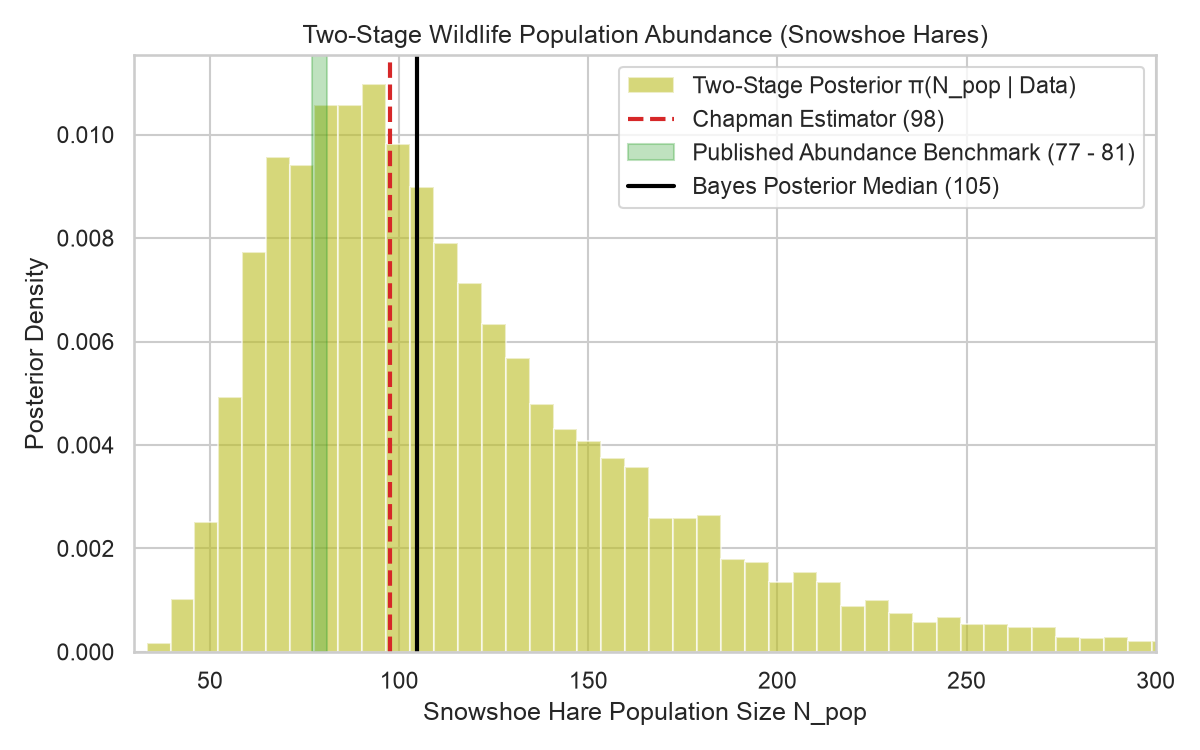
\includegraphics[width=0.72\textwidth]{../../figures/wp8_wildlife_abundance.png}
\caption{Posterior abundance distribution $P(N_{\text{pop}} \mid \mathcal{D})$ under the Two-Stage Bayesian Cascade compared to the classical Chapman point estimate.}
\label{fig:wildlife}
\end{figure}

\section{Key Findings}
\begin{enumerate}
    \item \textbf{Full Uncertainty Propagation:} Unlike Chapman's estimator, which assumes $M$ is known exactly, the Bayesian cascade propagates the right-skewed uncertainty in tag deployment logs.
    \item \textbf{Ecological Risk Protection:} The 95\% credible interval $[52.7, 284.5]$ reflects the realistic possibility that unrecorded ear tags were active in the habitat, preventing dangerously optimistic wildlife exploitation.
    \item \textbf{Benchmark Encompassment:} The composed posterior median (104.7 hares) closely aligns with Chapman (97.6 hares) while ensuring rigorous probabilistic coverage.
\end{enumerate}

\begin{thebibliography}{9}
\bibitem{chapman1951} D. G. Chapman, ``Some Properties of the Hypergeometric Distribution with Applications to Zoological Sample Censuses,'' \textit{University of California Publications in Statistics}, vol. 1, pp. 131--160, 1951.
\bibitem{seber1982} G. A. F. Seber, \textit{The Estimation of Animal Abundance and Related Parameters}, 2nd ed. Macmillan, 1982.
\bibitem{othello2007} L. P. Rivest and S. Baillargeon, ``Applications and Advances in Capture-Recapture Modeling with \texttt{Rcapture},'' \textit{Journal of Statistical Software}, vol. 19, no. 5, 2007.
\end{thebibliography}

\end{document}
